\chapter{Implementation of CCTVVS}

The implementation phase is significant phases in the project development as it
affords final solution that solves the issues. In this phase the low level
designs are transformed into the language specific programs such that the
requirements given in the software requirements specification are satisfied.
This phase entails actual implementation of ideas that were described in
analysis and design phase. The technique and the methods that are used for
implementing software must support reusability, ease of maintenance and should
be well documented.

\section{Modules and Classes}
We have split the code into different functional modules for easy development,
testing and maintenance of the code.

\begin{figure}[H]
    \centering
    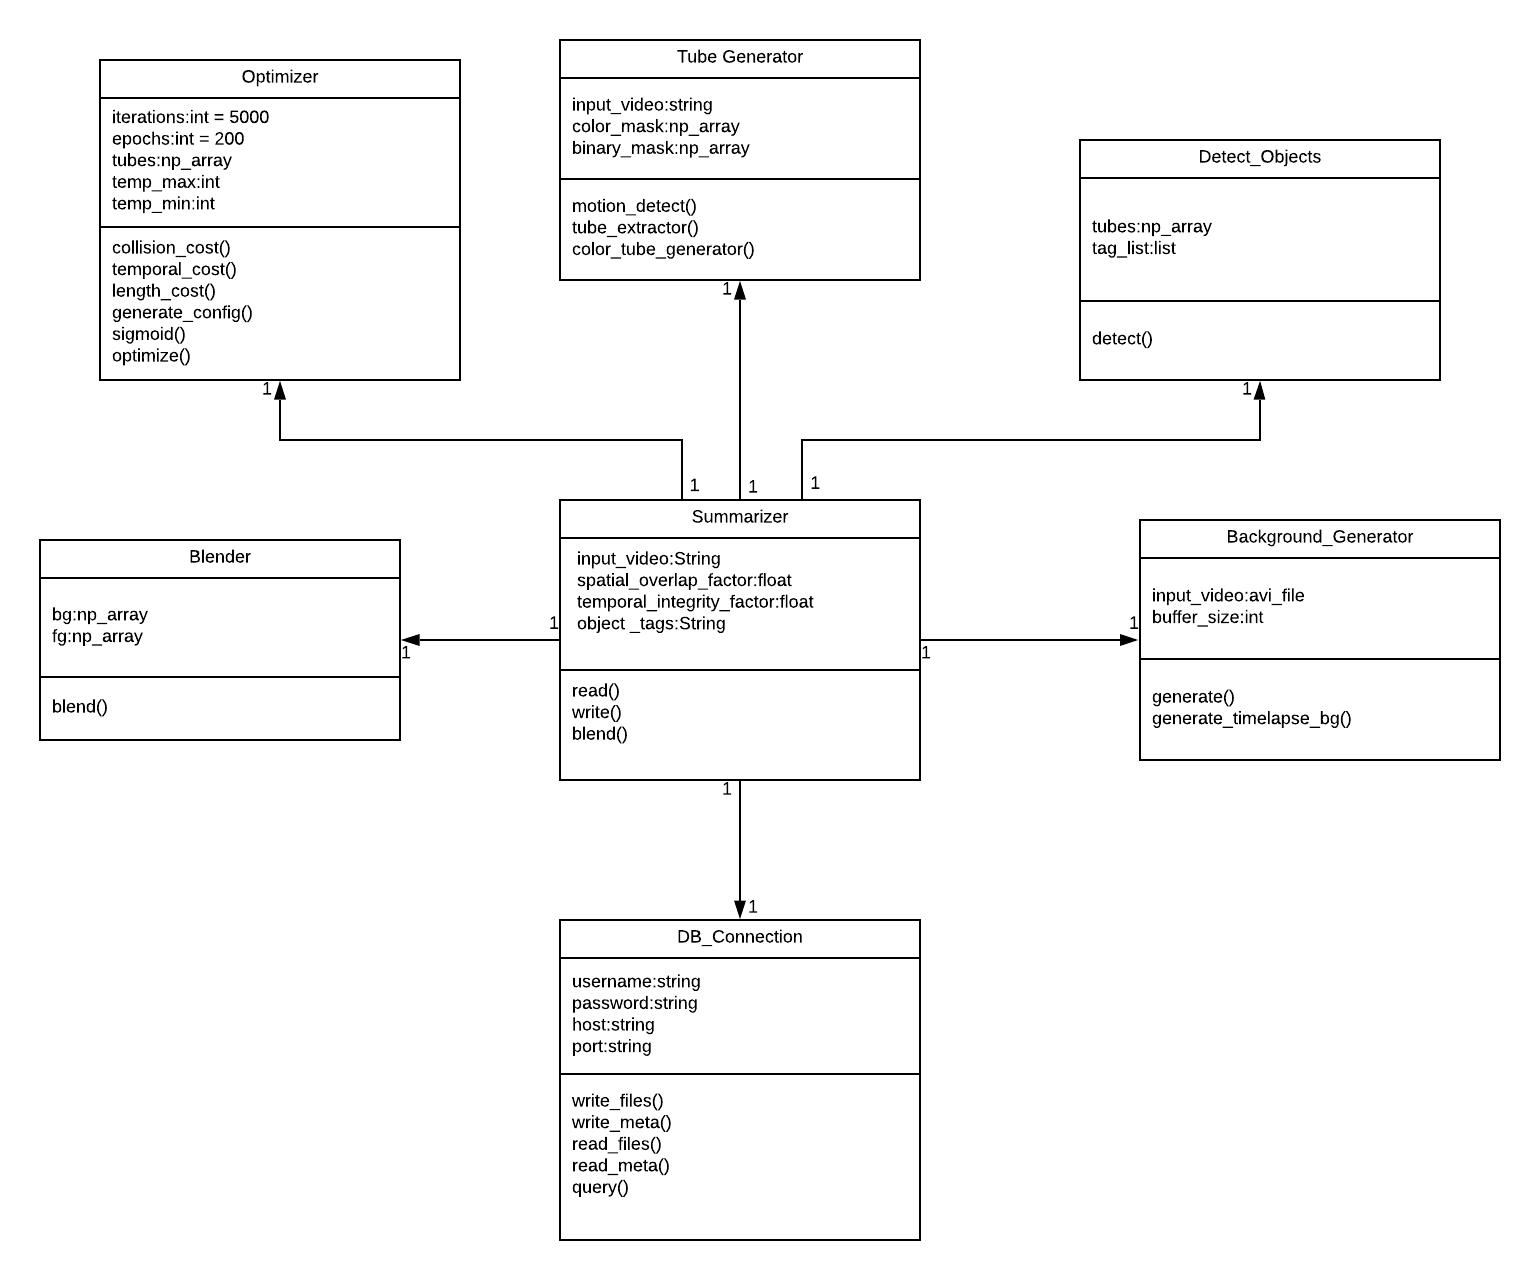
\includegraphics[scale=0.37]{uml.png}
    \caption{Classes / Modules of CCTVVS}
    \label{img:uml}
\end{figure}

The classes of the summarisation system are as shown in Figure \ref{img:uml}.
The central summariser object creates objects other modules mentioned in the
figure and uses them in a sequence mentioned in chapter 2. Each constructor of
the classes defined above, have strict assert statements to ensure the data they
receive are of the proper type before any kind of operations are performed on
them.

\section{Algorithms}

    \subsection{Simulated Annealing Algorithm}
    Algorithm \ref{algorithm:simulated-annealing} shows the simulated annealing algorithm
    which is used for the tube optimisation process.

    \begin{algorithm}
        \SetAlgoLined
        \KwResult{Optimised Configuration}
        Let \(Config_{current} = Config_{inital}\);
        \For {\(T \gets T_{max}\) \KwTo \(T_{min}\)}{
            \(E_{current} = E(C_{current})\)
            \(C_{next} = next(C_{current})\)
            \(E_{next} = E(C_{next})\)
            \(\Delta E = E_{next} - E_{curr}\)
            \uIf { \(\Delta E > \theta\)}{
                \(C_{current} \gets C_{next}\)
            }\uElseIf {\(e^{\frac{-\Delta E}{T}} > rand(0,1)\)}{
                \(C_{current} \gets C_{next}\)
            }
        }
        \caption{Simulated Annealing}
        \label{algorithm:simulated-annealing}
    \end{algorithm}

    \subsection{Tube Extraction Algorithm}
    Algorithm \ref{algorithm:tube-extraction} shows the tube extraction algorithm
    which is used for the extracting the event tubes from the labelled motion
    volume.

    \begin{algorithm}
        \SetKwInput{in}{input}
        \SetAlgoLined
        \KwResult{3D space-time volume with connected labelled events}
        \tcc{a 3d array representing the time-space volume with foreground
        represented as 1 and background as 0}
        \in{VideoMask}

        \(volume \gets empty\_list()\)
        \(tube\_num \gets 0\)
        \(prev\_frame \gets zeros\_like(VideoMask[1])\)
        \(prev\_count \gets 0\)

        \For {\(Frame in VideoMask\)}{
            \(labelled\_frame, count = findConnectedComponents(Frame)\)

            \For{\(i in range(0,count)\)} {
                \(matches \gets empty\_list()\)
                    \For{\(j in range(0, prev\_count)\)}{
                        \If { \(\frac{Sum((labelled\_frame[k==i]*prev\_frame))}
                        {Sum(prev\_frame)} > Threshold\) }{
                            \(matches.append(j)\)
                        }
                    }
                \(matches\_dict[i] \gets matches\)
            }

            \(prev\_frame \gets Frame\)
            \(prev\_count \gets count \)

            \For {\(region in match\_dict\)}{
                \If{\(len(match\_dict[region]) \textgreater 1\)}{

                    \For{\(index in match\_dict[region]\)}{
                        \For{\(frame in volume\)}{
                            \tcc{Update labels of tubes in previous frame}
                            \(frame[frame == index] = tube\_num\)
                        }

                        \tcc{Update the dict}
                        \(match\_dict[region] = [tube\_num]\)
                    }
                }
            }

            \tcc{There are no intersection issues; Proceed normally}
            \For {\(region in match\_dict\)}{
                \(cur\_img \gets labelled\_frame\)
                \(cur\_img\_output \gets labelled\_frame.clone()\)
                \(cur\_labels = empty\_list()\)
                \If {\(len(match\_dict[region]) == 0\)}{
                    \tcc{New region found since there is no match to any previous region}
                    \(tube\_num += 1\)
                    \(cur\_img\_output[cur\_img == region] = tube\_num\)

                }
                \Else{
                    \tcc{Some previous region was found, relabel the region}
                    \(cur\_img\_output[cur\_img == region] = match\_dict[region][0]\)
                }
            }
            \(volume.append(cur\_img\_output)\)
        }

        \caption{Tube Extraction}
        \label{algorithm:tube-extraction}
    \end{algorithm}

\section{Programming Language Selection}
The programming languages chosen to implement the project is Python. Python is
one of the most useful languages in the current age and time with extensive
support for fast development. Some of the benefits that Python provides which
were key for choosing the same are:

\begin{itemize}
    \item Simple, easy and highly readable program syntax
    \item Rapid development and prototyping process
    \item Jupyter notebook supports step-by-step execution of code for easier
    debugging
    \item Support of OpenCV wrapper
\end{itemize}


\section{Platform Selection}
The system has a basic user interface for the user input \& query, and the
backend system to process the input and generate the video summary. Python runs
on all 3 major computing platforms Windows, Linux and MacOS. The code has been
developed and tested on Windows and Mac platform using Python 3.6.

\section{Code Conventions}

This section discusses the coding standards followed throughout the project. It
includes the software applications that are necessary to complete the project.
Proper coding standards should be followed because large project should be coded
in a consistent style. This makes it easier to understand any part of the code
without much difficulty. Code conventions are important because it improves
readability in software, allowing the programmers to understand code clearly.

    \subsection{Naming Conventions}

    Naming conventions helps programs in understandable manner which makes
    easier to read. The names given to packages, scripts, graphs and classes are
    to be clear and precise so that their contents can easily be understood. The
    project uses both Java and Python, and the naming convention followed in the
    two are slightly divergent from each other.

    The conventions followed for this project are as follows:

    \begin{itemize}
        \item \textbf{Classes:} Class names are nouns. The upper camel casing
        method is followed, in which the first letter of every word is in
        capital, including the first word. Example: SimulatedAnnealing.
        \item \textbf{Methods:} Methods should be a verb. For methods, snake
        case is followed, where the names are in lowercase and multiple words
        are separated by underscores. Example: make\_summary()
        \item \textbf{Variables:} snake case is followed, where the names are
        in lowercase and multiple words are separated by underscores.
        Example: selected\_tubes
    \end{itemize}

    \subsection{File Organization}
    The code used to implement the project was organized into multiple files
    based on the functionality and the module to which the methods belonged.
    Each file contains a class which contains the required attributes and
    methods.
    Ex: SimulatedAnnealing class contains attributes like T\_max, T\_min,
    iterations etc and methods like calc\_cost(), optimize() etc


    \subsection{Declarations}

    Standard declaration conventions are followed while coding. Standard names
    are given which make it easy to understand the role of each entity declared.
    Multiple declarations per line are not allowed because of commenting and to
    reduce ambiguity.

    \subsection{Comments}
    Comments are necessary part of any coding conventions as it improves the
    readability of the code developed. In the project files, thanks to the
    integrated development environments, commented areas are printed in grey by
    default, so they are easy to identify.
    In Python comments start with a ‘\#’. There are keyboard shortcuts and
    mouse options provided to comment out or uncomment blocks of code with ease.
    Comments are used for explaining what function a certain piece of code
    performs especially if the code relies on implicit assumptions or otherwise
    perform subtle actions.

\section{Difficulties Encountered and Strategies Used to Tackle}
This section discusses some of the difficulties encountered while developing
this project.

    \subsection{Static Background Generation}
    The system has to generate a static background from the moving background,
    and a temporal median is proposed for the same. Since the same was
    computationally intensive, the Mixture of Gaussians in OpenCV has been used
    for estimating the static background, which performs better.

    \subsection{Simulated Annealing}
    The video summariser optimizes the tubes which are extracted from the input
    video, and this is a NP-complete problem, where every single
    possibility can't be examined. A heuristic based optimization algorithm such
    as simulated annealing is required. A set of cost functions have been
    created which calculate the collision cost and length cost, which are used
    by the optimization algorithm. Simulated annealing, which is a probabilistic
    technique, is used for estimating the global optimum. The cost of a
    configuration is evaluated and then the decision to update the configuration
    is based on other parameters. The simulated annealing algorithm is
    optimised by using a resized image, and by parallelising it for faster
    processing.

\section{Summary}
This chapter deals with the programming language used which is Python, the
development environment and the code conventions followed in the two languages
during implementation of the application. It also explains the difficulties
encountered in the course of implementation of the system like background
generation and simulated annealing and the strategies used to handle them.